В данной задаче прогнозировалось количество фильмов по жанрам на 10 лет. Сразу стоит отметить, что рассматривались только фильмы до 2019-го года включительно, так как из-за пандемии коронавируса в 2020-ом году количество фильмов резко сократилось. Поэтому прогнозируется количество фильмов по жанрам, если бы в 2020-ом году не было пандемии коронавируса. В основном, для всех жанров прогнозируется продолжение роста количества фильмов - примером явлются мультфильмы (см. Рис.~\ref{fig:cartoons}). Но встречаются и редкие жанры, для которых на основе чередования роста и снижения количества фильмов в последнее время спрогнозировалось продолжение этого чередования - примером является жанр фэнтези (см. Рис.~\ref{fig:fantasy}).

\begin{figure}[ht!]
	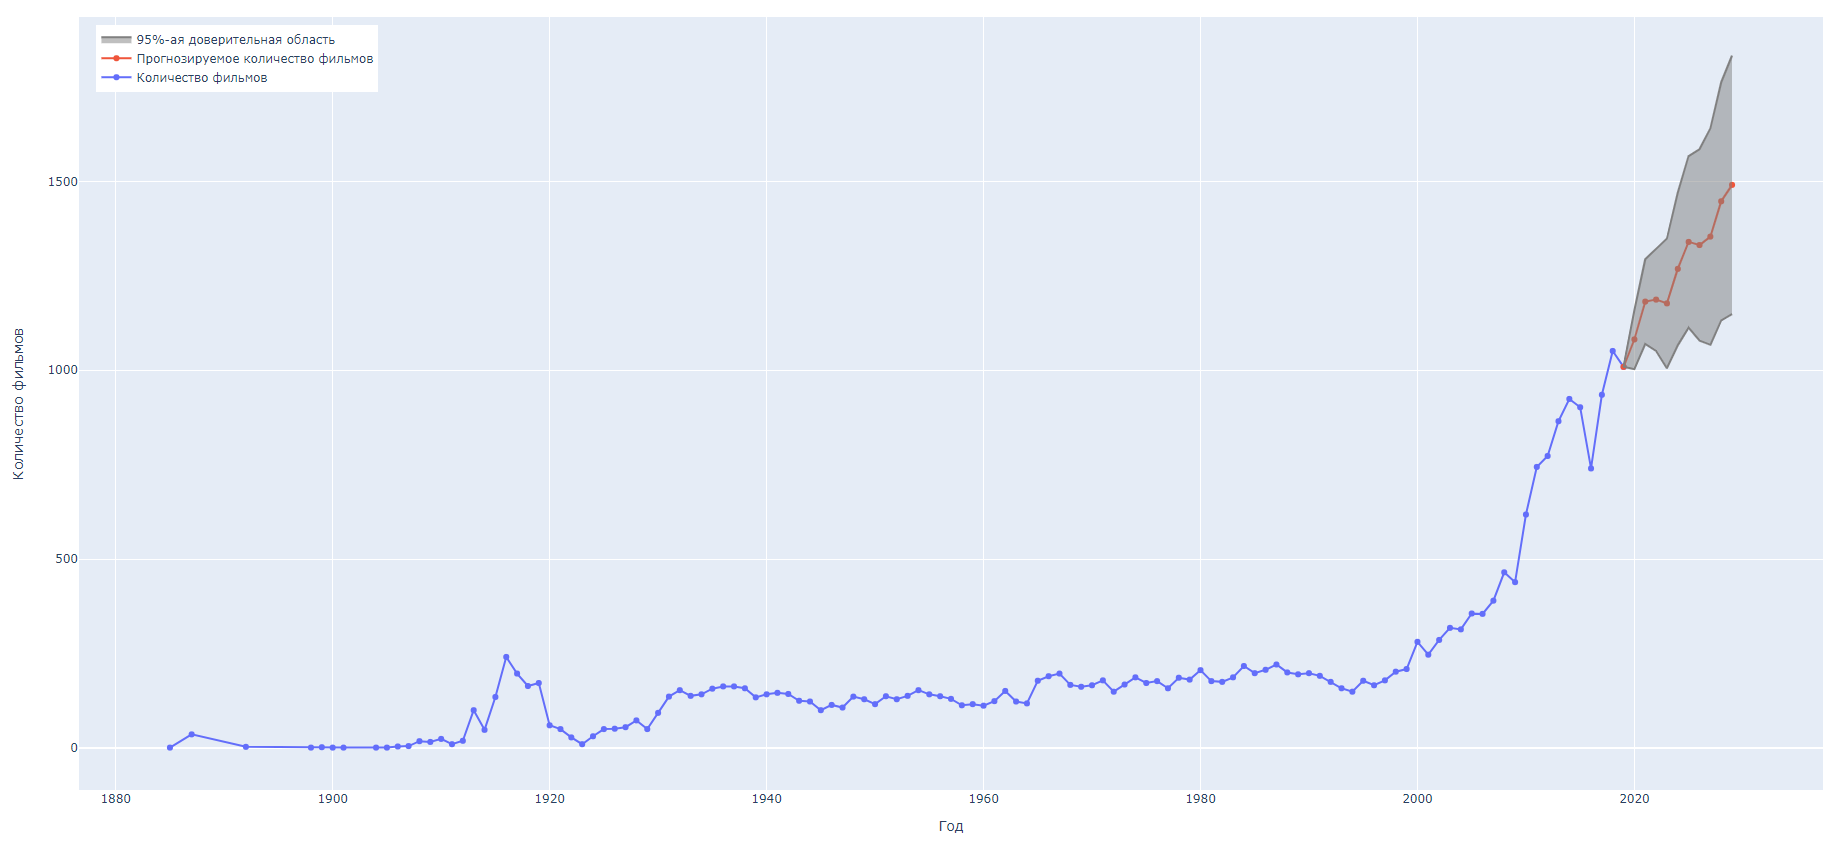
\includegraphics[width=\linewidth]{../report/images/genre_predict/cartoons}
	\caption{Прогноз количества мультфильмов на 10 лет.}
	\label{fig:cartoons}
\end{figure}

\begin{figure}[ht!]
	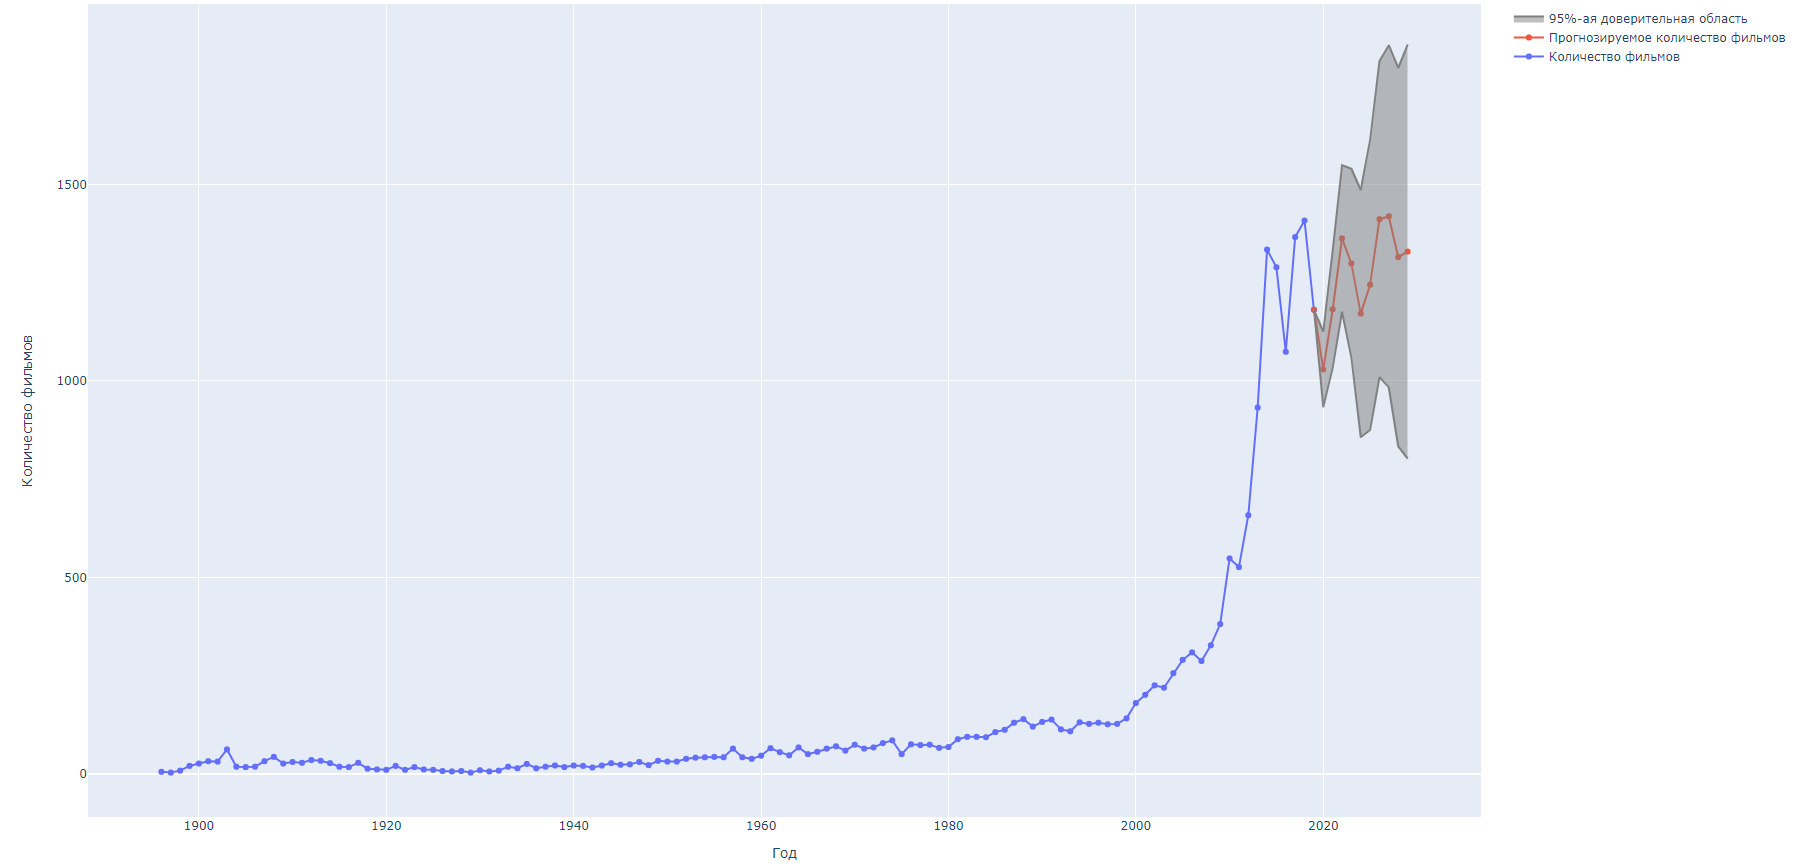
\includegraphics[width=\linewidth]{../report/images/genre_predict/fantasy}
	\caption{Прогноз количества фильмов жанра фэнтези на 10 лет.}
	\label{fig:fantasy}
\end{figure}



